%%%%%%%%%%%%%%%%%%%%%%%%%%%%%%%%%%%%%%%%%%%%%%%%%%%%%%%%%%%%%%%%%%%%%%%%%%%%%%%%%%%%%%%%%%%%%%%%%%%%%%%%%%%%%%%%%%%%%%%%%%%%%%%%%%%%%%%%%%%%%%%%%%%%%%%%%%%%%%%%%%%%%%%
%%%%%%%%%%%%%%%%%%%%%%%%%%%%%%%%%%%%%%%%%%%%%%%%%%%%%%%%%%%%%%%%%%%%%%%%%%%%%%%%%%%%%%%%%%%%%%%%%%%%%%%%%%%%%%%%%%%%%%%%%%%%%%%%%%%%%%%%%%%%%%%%%%%%%%%%%%%%%%%%%%%%%%%
\chapter{Optimisation of the search sensitivity}
\label{sec:Optimisation}
Finally, having all background estimation methods in place, an optimisation procedure is conducted to increase the search sensitivity with respect to the signal models introduced in Section~\ref{sec:SignalSamples}.
The optimisation is done in the most sensitive variables, \pt and \ias.
In this optimisation, the full systematic uncertainty is taken into account, which includes statistical uncertainties arising from limited statistical precision of the samples used in the background estimation methods and the systematic uncertainties that are described in Section~\ref{sec:SysUncertaintiesBkg}.
In order to avoid unnecessary fine-tuning of the optimisation to the specific cross sections of the SUSY models and to keep the search as general as possible, 
the optimisation is not done by maximising  $S/\Delta B$ but by minimising the cross section for which a 5$\sigma$ discovery is possible
\begin{equation}
\label{eq:optimisation}
\frac{\sigma_{\text{min}}\cdot \mathcal{L}}{\Delta B} = \frac{\sigma_{\text{min}}\cdot \mathcal{L}}{\sqrt{ \Delta B_{\text{stat}} + \Delta B_{\text{sys}}}} \geq 5.
\end{equation} 
In this formula, $\mathcal{L}$ is the integrated luminosity in 2012, $\sigma_{\text{min}}$ is the cross section to be minimised, $\Delta B_{\text{sys}}$ is the systematic uncertainty of the background prediction as explained above and 
$\Delta B_{\text{stat}}$ is the statistical uncertainty of the background prediction which is the 68\% one sided upper limit of a poisson distribution with $\mu = B$ estimated with the 
Neyman construction~\cite{bib:Neyman_1937,bib:PDG_2014}.

Four different benchmark models are choosen for the optimisation.
As this analysis focus on short tracks, models with charginos with low lifetimes are choosen: $\ctau=1\cm$ and $\ctau=5\cm$. 
Additionally, two different masses in order to cover also the mass dimension: 100\gev and 500\gev.

A visualised optimisation is done by imposing general systematic uncertainties on the leptonic and the fake background of 100\% and 20\% respectively whereas
the uncertainties arising from limited statistical precision of the samples are propagated accurately into the formula~\ref{eq:optimisation}.
The results can be found in Fig.~\ref{fig:optimisation}, where the minimal cross section that is possible to exclude is shown in the $\pt-\ias$ plane.
\begin{figure}[!h]
  \centering 
  \begin{tabular}{c}
    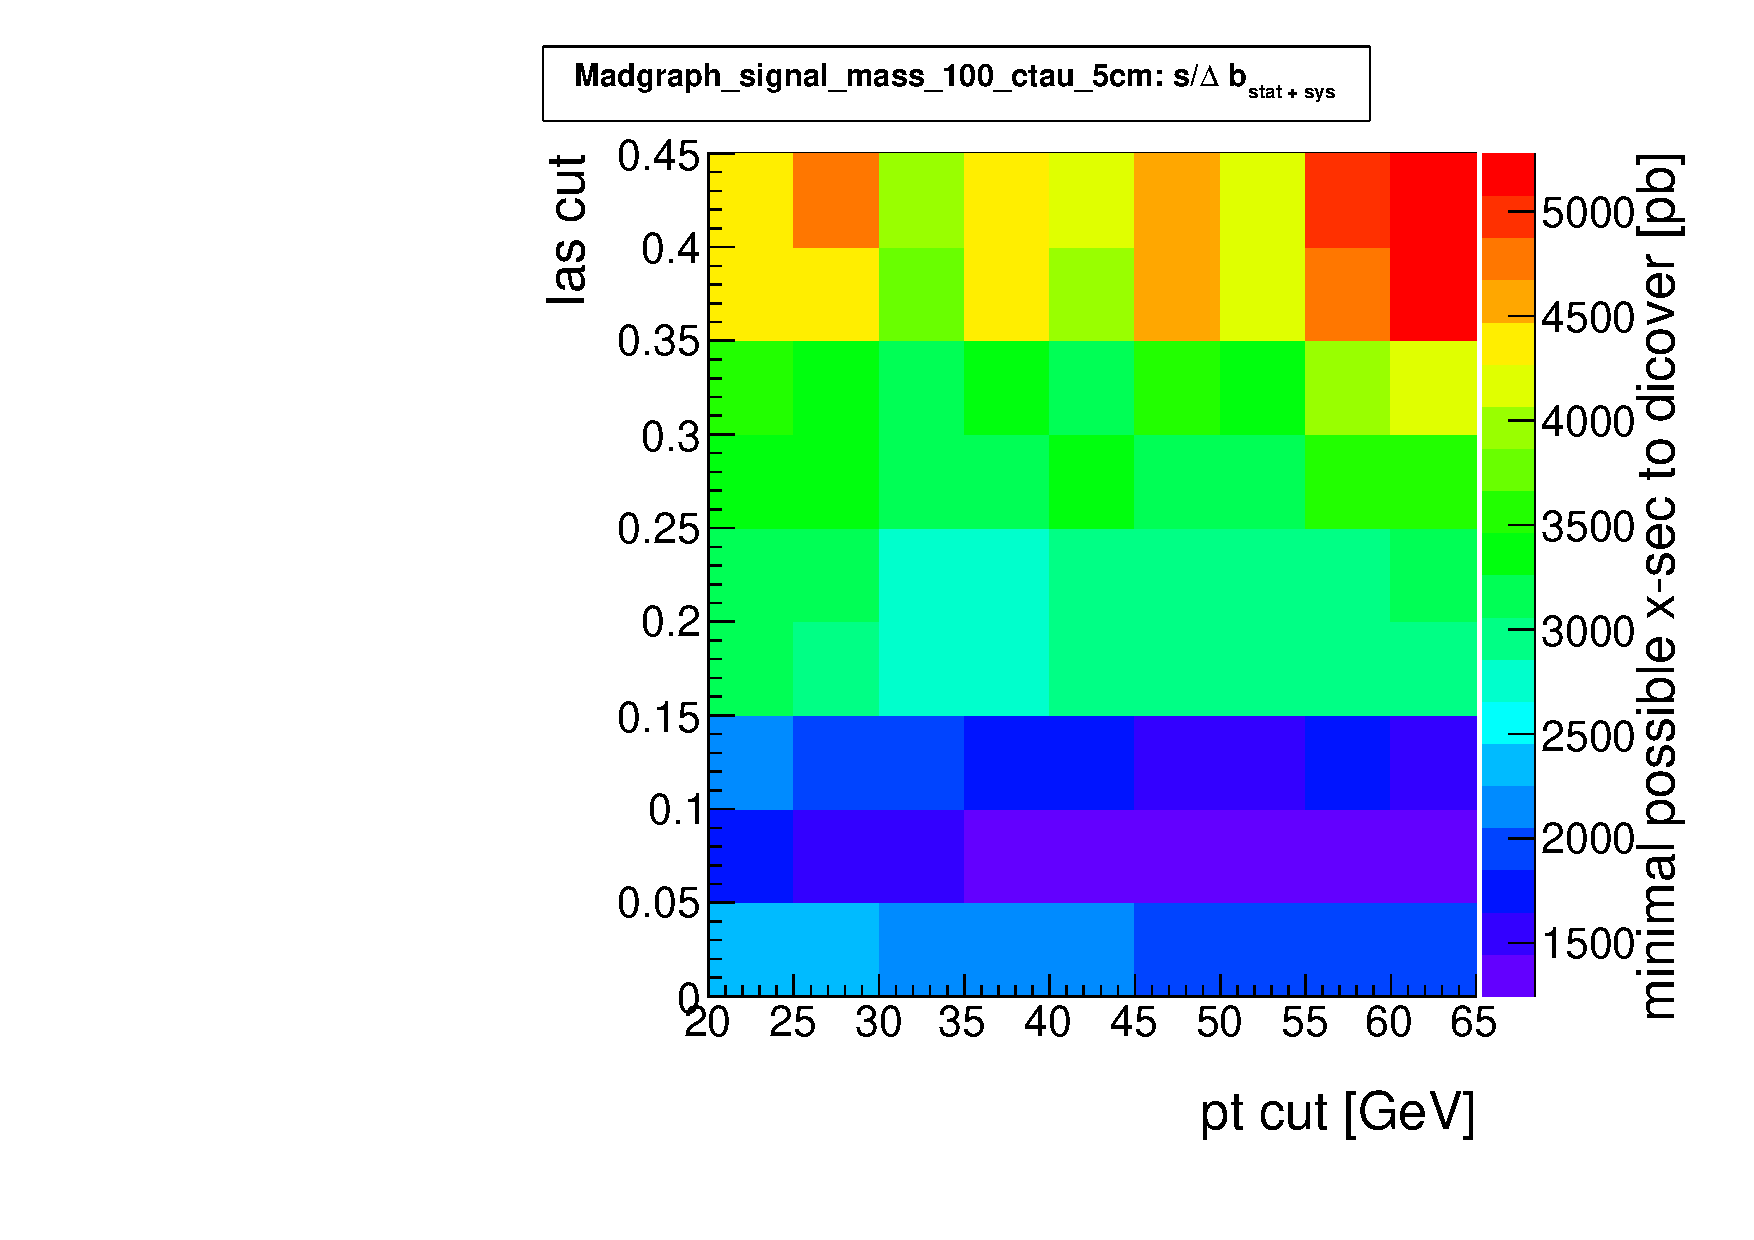
\includegraphics[width=0.49\textwidth]{figures/analysis/Optimisation/Madgraph_signal_mass_100_ctau_5cm_ECaloLe5_SOverDeltaBStatPlusSys.pdf} 
    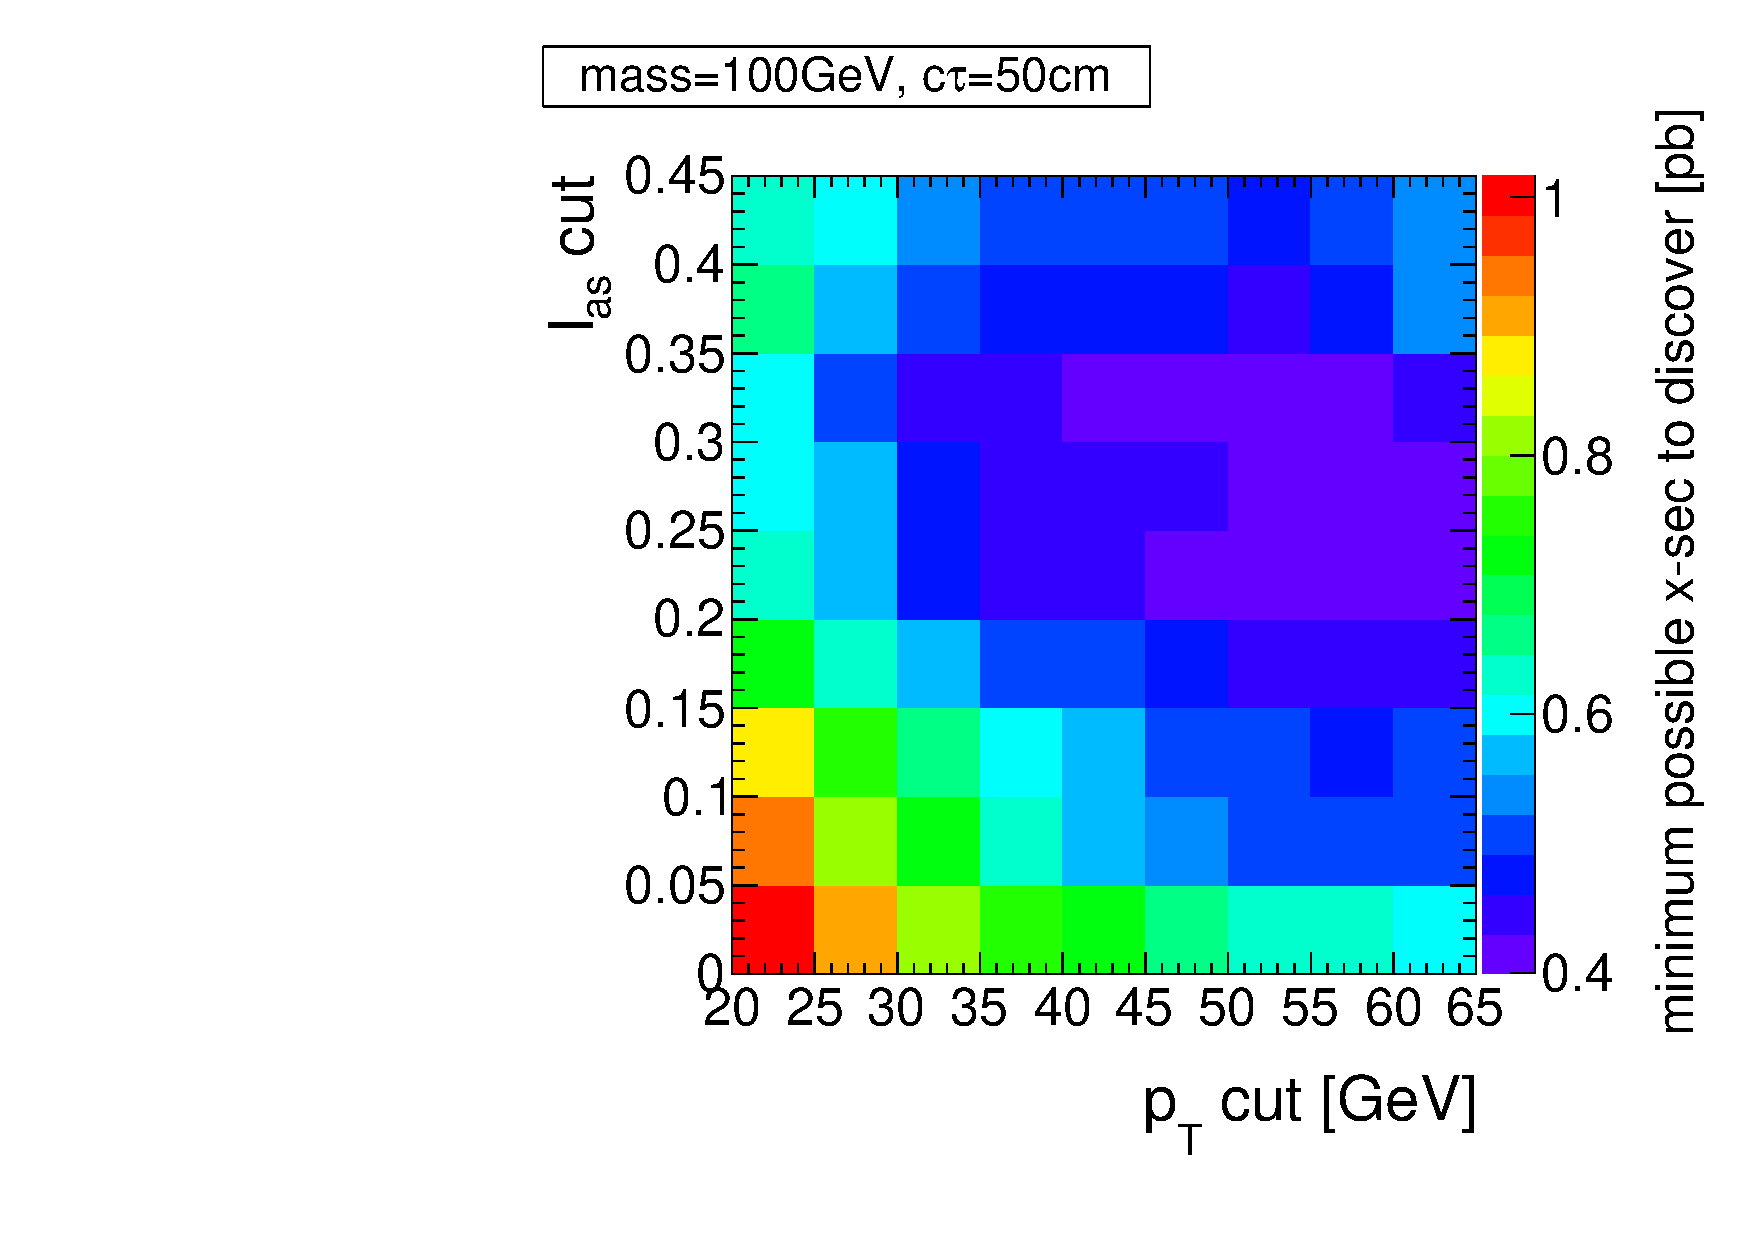
\includegraphics[width=0.49\textwidth]{figures/analysis/Optimisation/Madgraph_signal_mass_100_ctau_50cm_ECaloLe5_SOverDeltaBStatPlusSys.pdf}\\ 
    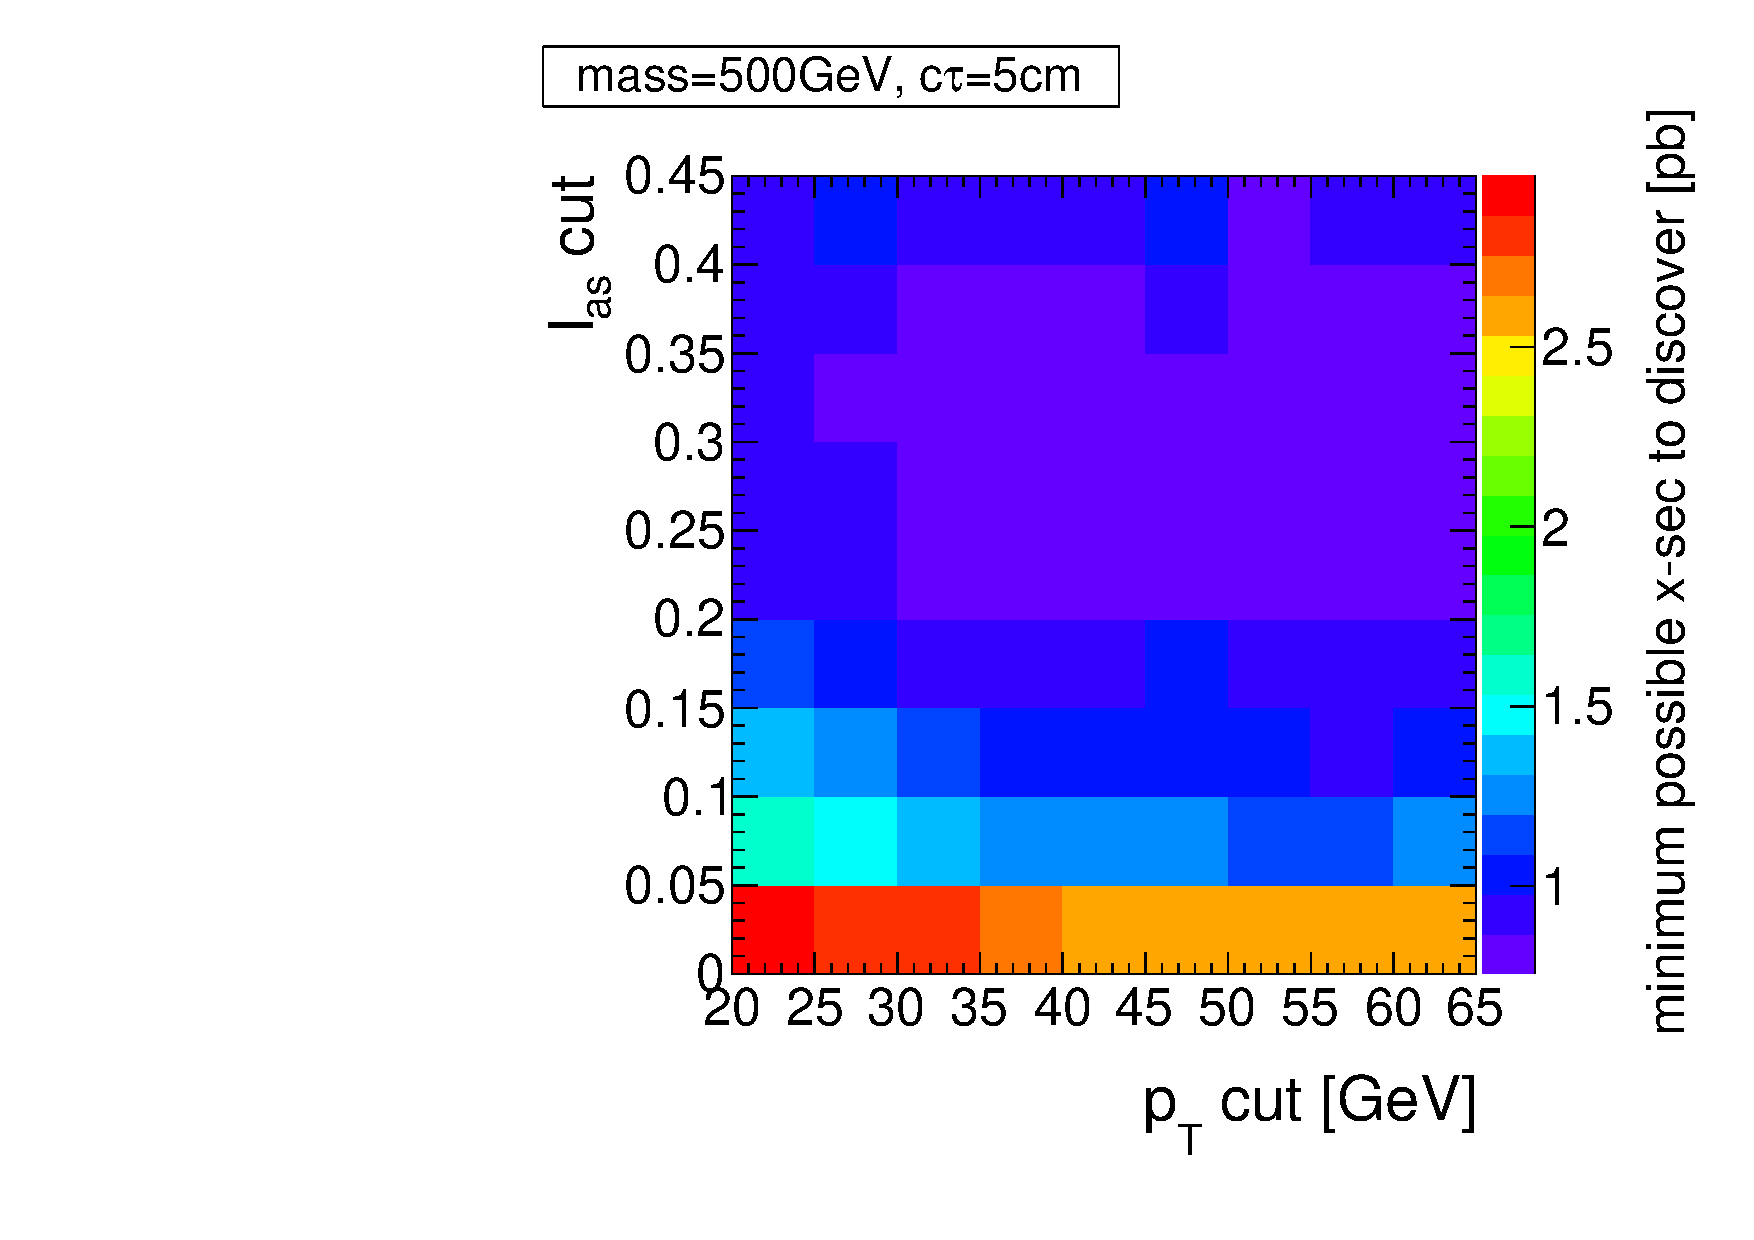
\includegraphics[width=0.49\textwidth]{figures/analysis/Optimisation/Madgraph_signal_mass_500_ctau_5cm_ECaloLe5_SOverDeltaBStatPlusSys.pdf}
    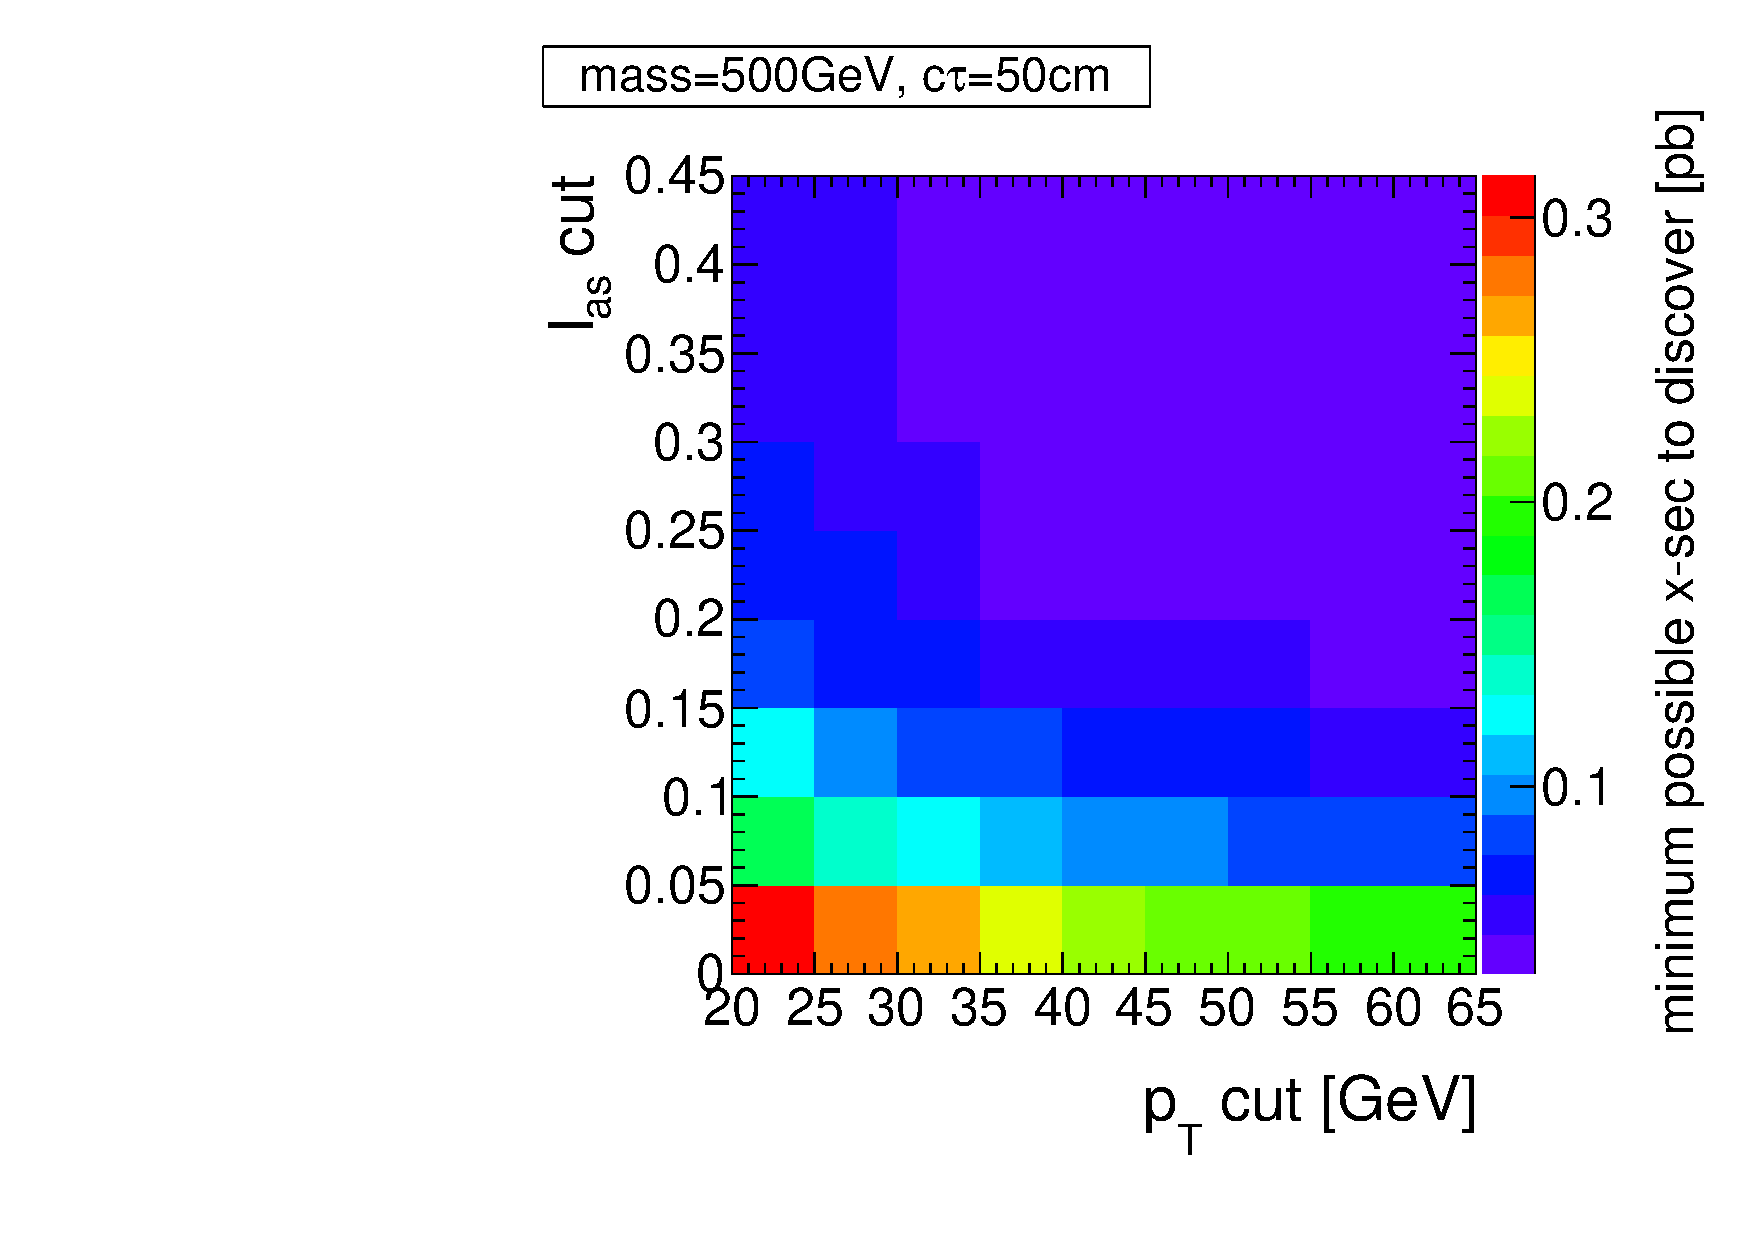
\includegraphics[width=0.49\textwidth]{figures/analysis/Optimisation/Madgraph_signal_mass_500_ctau_50cm_ECaloLe5_SOverDeltaBStatPlusSys.pdf} 
  \end{tabular}
  \caption{Minimal possible cross section to exclude in the $\ias-\pt$ plane for four different signal models.}
  \label{fig:optimisation}
\end{figure} 
A exact optimisation taken the whole background uncertainties precisly into account is done without a visualisation.
The corresponding results are shown in Table~\ref{tab:optimisation}.

\renewcommand{\arraystretch}{1.5}
\begin{table}[!h]
\centering
\caption{Optimal \pt and \ias cuts and corresponding minimal possible cross section $\sigma_{\text{min}}$ to exclude for different signal models.}
\label{tab:optimisation}
\makebox[0.99\textwidth]{
\begin{tabular}{c |c| c| c| c}
\multicolumn{5}{c}{} \\
\toprule
Mass [\gev] & Lifetime [\cm] & Optimal \pt cut & Optimal \ias cut & $\sigma_{\text{min}}$ \\
\midrule
100&                           1&                             30&                            0.05&                          59.0291   \\
500&                           1&                             0 &                            0.0 &                          10000.0000\\
100&                           5&                             50&                            0.05&                          2.6965    \\
500&                           5&                             50&                            0.30&                          0.6180    \\
\bottomrule
\multicolumn{5}{c}{} \\
\end{tabular}}
\end{table}

It can be seen that the optimal selections are highly dependent on the signal models.

Additionally, it is checked whether a sensitivity increase can be achieved by imposing also a selection on the number of missing outer hits $N_{lost}^{outer}$.
For low lifetimes, a tiny increase in sensistivy is possible by selecting also in this variable but as this variable comes with new sources of uncertainties this is not consideres in this search.

To have an optimal coverage over a wide mass space, four different signal regions are defined:
\begin{enumerate}
\item $30\gev<\pt<50\gev$ and $0.05<\ias<0.3$
\item $30\gev<\pt<50\gev$ and $\ias>0.3$
\item $\pt>50\gev$ and $0.05<\ias<0.3$
\item $\pt>50\gev$ and $\ias>0.3$.
\end{enumerate}

%%%%%%%%%%%%%%%%%%%%%%%%%%%%%%%%%%%%%%%%%%%%%%%%%%%%%%%%%%%%%%%%%%%%%%%%%%%%%%%%%%%%%%%%%%%%%%%%%%%%%%%%%%%%%%%%%%%%%%%%%%%%%%%%%%%%%%%%%%%%%%%%%%%%%%%%%%%%%%%%%%%%%%%
%%%%%%%%%%%%%%%%%%%%%%%%%%%%%%%%%%%%%%%%%%%%%%%%%%%%%%%%%%%%%%%%%%%%%%%%%%%%%%%%%%%%%%%%%%%%%%%%%%%%%%%%%%%%%%%%%%%%%%%%%%%%%%%%%%%%%%%%%%%%%%%%%%%%%%%%%%%%%%%%%%%%%%%
\chapter{Results}
\label{sec:Results}

\begin{itemize}
\item correlations between signal regions
\item Data cutflowtable
\item Tables with results
\item One plot (4 bins: Prediction and data)
\end{itemize}

%%%%%%%%%%%%%%%%%%%%%%%%%%%%%%%%%%%%%%%%%%%%%%%%%%%%%%%%%%%%%%%%%%%%%%%%%%%%%%%%%%%%%%%%%%%%%%%%%%%%%%%%%%%%%%%%%%%%%%%%%%%%%%%%%%%%%%%%%%%%%%%%%%%%%%%%%%%%%%%%%%%%%%%
%%%%%%%%%%%%%%%%%%%%%%%%%%%%%%%%%%%%%%%%%%%%%%%%%%%%%%%%%%%%%%%%%%%%%%%%%%%%%%%%%%%%%%%%%%%%%%%%%%%%%%%%%%%%%%%%%%%%%%%%%%%%%%%%%%%%%%%%%%%%%%%%%%%%%%%%%%%%%%%%%%%%%%%

\chapter{Interpretation}
\label{sec:Interpretation}
\section{Systematic uncertainties of simulated signal samples}
\section{Statistical Methods/ Limit setting}
\section{Exclusion limits}
\begin{itemize}
\item 1-d limits
\item 2-d limits
\end{itemize}


\chapter{Discussion and outlook and conclusion}
\label{sec:Discussion}
